\documentclass{article}
\usepackage{amsmath,amssymb}
\usepackage[utf8]{inputenc}
\usepackage{graphicx}
\usepackage{hyperref}
\usepackage{mathrsfs}
\usepackage{mathtools} 
\usepackage{mathrsfs} 
\usepackage{dsfont}
\usepackage{float}
\usepackage{subcaption}
%\usepackage{authblk}
%\usepackage{pdftex}
\usepackage{tikz}
\usepackage{booktabs, multirow} % for borders and merged ranges
\usepackage{soul}% for underlines
%\usepackage[table]{xcolor} % for cell colors
\usepackage{changepage,threeparttable} % for wide tables
\usepackage[font=small]{caption}
\usepackage[a4paper]{geometry}
\usepackage[round,comma,numbers,authoryear]{natbib}
\hypersetup{colorlinks,urlcolor=blue, linkcolor=blue, citecolor = blue}
\usepackage{cleveref}
\usepackage{enumerate}
\usepackage[]{caption} 
\captionsetup[table]{skip=1pt}
\usepackage[]{threeparttable}
\usepackage{subcaption}
\usepackage{comment}
\captionsetup[subfigure]{subrefformat=simple,labelformat=simple}
\renewcommand\thesubfigure{(\alph{subfigure})}
\DeclareMathOperator*{\argmax}{argmax}
%=====================================================================


%\author{Hassan Sadeghi\thanks{Department of Finance, University of Zurich. hassan.sadeghi@uzh.ch} \and Mohsen Mohaghegh\thanks{Department of Economics, Indian Institue of Management Ahmedabad. mohsenm@iima.ac.in.}}

\geometry{
a4paper,
top=2cm,
left=2.5cm,
right=2.5cm
}
\begin{document}
\title{The Asymmetry of Conditional Dependence Structures in the Cryptocurrency Market}

\maketitle
%=====================================================================
\begin{abstract}
We design a quantile measure of conditional tail asymmetry and use it to examine dependence structures in the cryptocurrency and the equity market. We find that conditional tail asymmetry is significantly stronger in cryptocurrencies. This happens because cryptocurrencies have largely weaker right-tail correlations while their left-tail dependence is more pronounced, indicating a higher systemic risk in that market. We also find that conditional tail asymmetry in the equity market is mostly found in tails that only include very extreme returns. We show that this asymmetry substantially weakens as the quantile tail criterion rises. In the cryptocurrency market, however, tail asymmetry remains significantly large throughout the entire joint distribution of returns. We verify the robustness of our findings through a series of parametric bootstraps.\par  
\end{abstract}
%=====================================================================

\section{Introduction}
In only 15 years since the introduction of Bitcoin, the global market capitalization of cryptocurrencies has already surpassed 2.5 trillion USD in 2024. This surge has captured the attention of many researchers. Though some studies merely consider cryptocurrencies as alternatives to traditional financial instruments -\textit{e.g.,} equities- \citep{guesmi2019, Bouri2020, wen2022}, their rising importance has brought to the center their returns' dynamics as well as their relationship with one another \citep{liu2019, li2022}. From this literature, we know that, despite many similarities, there are consequential differences between equities and cryptocurrencies. For example, cryptocurrencies have heavier tails \citep{Gkillas2018} and are more volatile \citep{fung2021, malek2023} than the equities. We highlight another difference between the equity market and the cryptocurrency market as related to the tail conditional dependence structures.  \par

It is well known that correlations between equities are greater during extreme downside moves than upswings \citep{longin2001, ang2002asymmetric}. This so-called `asymmetry' results in strong(er) left-tail correlations compared to right-tail correlations in the equity market. Overall, similar relations have been reported in cryptocurrencies \citep{feng2018, li2022}.\footnote{\cite{ahn2022} also provide empirical evidence for the asymmetry of conditional correlations between three cryptocurrencies and the S\&P 500 index.} However, there are idiosyncrasies in the cryptocurrency market that have inspired considering nonlinear \citep{li2022} and time-varying \citep{aslanidis2019, wang2022} correlation models. Understanding tail dependence structures is crucial for the investors as well as the regulators because they have important implications for portfolio management \cite{sleire2022portfolio} and directional predictions \cite{bekiros2021}. We contribute to this literature by identifying two differences in the pattern of tail asymmetries between the cryptocurrency and the equity market.\par

Our sample, based on market capitalization, includes the ten largest cryptocurrencies and the five largest companies in each of the eleven sectors of the S\&P 500. For each pair, we compute the difference between left-tail and right-tail correlations of assets conditional to a quantile tail criterion. A small quantile tail criterion implies that the tail only includes extreme returns while for larger values of this quantile tail criteria less extreme returns are also considered. Thus, by changing this criterion, one can capture the evolution of tail asymmetry in both markets. We call this measure `Conditional Quantile Correlation Difference (CQCD)', and compute it for different tail criteria based on the Kendall's rank correlation in both markets.\par 

We find that conditional correlation between assets on the lower-left tail of their joint distribution (in short, left-tail correlations) are by and large stronger in the cryptocurrency market compared to the equity market. On the contrary, conditional correlations between assets on the upper-right tail of their joint distribution (in short, right-tail correlations) are stronger in the equity market. As a result, tail asymmetry is significantly stronger between cryptocurrencies. For instance, when the tail criterion is such that only five percent of the data on each tail is considered, the average CQCD in cryptocurrencies, $0.30$, is noticeably greater than its average between the equities, $0.02$. This quantitative difference between the two markets is the first result of our paper for which we provide more evidence in the paper. We also show that the asymmetry between conditional correlations in the equity market substantially weakens as the tail criterion rises while in the cryptocurrency market, it remains significantly large over the entire joint distribution of assets. For instance, if we raise the tail threshold so that instead of five, up to fifteen percent of the data on each tail is considered, the proportion of equity pairs for which conditional tail asymmetry (CQCD) is less than $0.10$, on average, increases from $57$ to $79$ percent as opposed to the cryptocurrency market where this ratio remains almost unchanged at about $0.4$ percent. Even after doubling the tail threshold, this proportion in cryptocurrencies does not increase while in equities, it reaches to over $85$ percent. After empirically establishing both patterns, we run a series of parametric bootstraps where we capture the joint distribution of each pair by fitting a bivariate copula to the data, and use that for random sampling. The resulting synthetic bootstrap-generated measures of tail asymmetry confirm both our findings. \par 
The remainder of the paper is organized as follows. Section \ref{model} reviews our methodology. Section \ref{data} introduces the data. Section \ref{res} presents our findings. Finally, Section \ref{con} concludes.

\section{Methodology}\label{model}
The conditional right-tail and left-tail correlations are usually defined as the correlation between two assets on a subspace of their mutual return distribution where \textit{both} returns satisfy a tail criterion as formally given by \ref{def1}: 
\vspace{-2mm}
\begin{align}\label{def1}
\begin{split}
\tau_{ij}^{+}(\alpha) &\equiv  \text{Corr}\Big(r_{i,t}, r_{j,t} \hspace{1mm} \Big| \hspace{1mm} r_{i,t} > F^{-1}_{r_{i}}(\alpha) \hspace{1mm} , \hspace{1mm} r_{j,t} > F^{-1}_{r_{j}}(\alpha)\Big)  \\[1.5mm]
\tau_{ij}^{-}(\alpha) &\equiv \text{Corr}\Big(r_{i,t}, r_{j,t} \hspace{1mm} \Big| \hspace{1mm} r_{i,t} < F^{-1}_{r_{i}}(\alpha) \hspace{1mm} , \hspace{1mm} r_{j,t} < F^{-1}_{r_{j}}(\alpha)\Big)  
\end{split}
\end{align}

\noindent where the return series \( r_{t} \in \mathbb{R}, \; t = 1, \dots, T \) has a CDF, \( F_{r}(\cdot) \), and quantile function, \( F^{-1}_{r}(\cdot) \). According to this definition, the correlations are computed when both returns are higher (or lower) than their $\alpha^{\text{th}}$ percentile of their respective distributions.\footnote{In this paper, We measure and report the correlation between assets using Kendall's $\tau$. We have also computed all our measures of tail asymmetry using the Pearson's correlation coefficient. Our findings are not sensitive to this change. These results are available upon request.}. The idea of asymmetric tail dependence structures, then, implies that the assets are more correlated when both are performing poorly compared to when both are performing well; \textit{i.e.,} $\tau_{ij}^{-}(1) > \tau_{ij}^{+}(99)$.\par

We, however, use a slightly different definition. The main difference is that the second measure only requires one of the assets to satisfy the tail criterion and there are no requirements for the other as demonstrated in \ref{def2}:

\vspace{-2mm}
\begin{equation}\label{def2}
\begin{split}
\tilde{\tau}^{i,+}_{ij}(\alpha) &\equiv \text{Corr}\Big(r_{i,t}, r_{j,t} \hspace{1mm} \Big| \hspace{1mm} r_{i,t} > F^{-1}_{r_{i}}(\alpha) \Big)  \\[1.5mm]
\tilde{\tau}^{i,-}_{ij}(\alpha) &\equiv \text{Corr}\Big(r_{i,t}, r_{j,t} \hspace{1mm} \Big| \hspace{1mm} r_{i,t} < F^{-1}_{r_{i}}(\alpha)\Big)  
\end{split}
\end{equation}

We use this definition for both empirical and conceptual reasons.\footnote{We have computed all the measures of tail asymmetry with the first definition as well. Our finding are robust to this change. These results are available upon request.} First, the fact that no restrictions are imposed on the second asset implies that, in any sample, the number of observations that satisfy the second definition in \ref{def2} is greater than or equal to those that satisfy \ref{def1}. This is an empirical advantage for studying tail structures where usually the sample size is small. Second, conceptually, the first definition aims to capture dependence structures in different market conditions as it requires both assets to meet the tail criterion. For instance, when both assets have high returns, the the overall market condition is likely to favorable. Similarly, when both are performing poorly, we are likely to be in a bear market. The second definition, however, simply captures asset $j$'s response to unusually high or low returns of asset $i$, regardless of the overall market conditions. This is more intuitive for risk and portfolio management as the investors' interest in diversification is not limited to the times of crisis only. As a caveat, the second definition is not symmetric as there is no reason to conclude that $\tilde{\tau}^{i,+}_{ij}(\alpha) = \tilde{\tau}^{j,+}_{ij}(\alpha)$. This increases the computational burden of applying this definition to a large number of assets. 


\subsection{Conditional Quantile Correlation Difference}\label{sec:cqcd}

To quantify the asymmetry in tail dependence structures between two assets, we compute a relative measure of conditional dependence, which we call `Conditional Quantile Correlation Difference (CQCD)'. The CQCD, for a pair of assets and a tail quantile criterion $\alpha \in (0, 50)$, is defined as the difference between two conditional correlations:

\vspace{-3mm}
\begin{align}\label{def3}
\mathbb{C}^i_{ij}(\alpha) \equiv \tilde{\tau}^{i,-}_{ij}(\alpha) \hspace{1mm} - \hspace{1mm} \tilde{\tau}^{i,+}_{ij}(100-\alpha)
\end{align}

This measures the difference between the assets' correlation over the lowest $\alpha$ percentiles of the return of asset $i$, and their correlation over the highest $\alpha$ percentiles of the return of asset $i$. When $\alpha$ is close to zero, we are only considering a small segment of the joint distribution that contains extreme returns of asset $i$ on each tail. As $\alpha$ increases, less extreme returns are also included so that $\alpha = 50$ covers the entire joint distribution. It is worth noting that this measure of conditional asymmetry is not symmetric; \textit{i.e.,} $\mathbb{C}^i_{ij} (\alpha) \neq \mathbb{C}^j_{ij}(\alpha)$. 


\subsection{Parametric Bootstrap Algorithm}\label{sec:boot}

The steps, for each pair, include: 

\begin{enumerate}[I)]
    \item \textbf{Converting Returns to Pseudo-observations:} For each asset $i \in \{1,2\}$, compute pseudo-observations from the return series \( r_{i,t} \in \mathbb{R}, \; t = 1, \dots, T \), such that each element is represented as \( u_i = F_{r_i}(r_{i,t}) \), where \(F_{r_i}\) is the empirical distribution function of returns and $ u_i \sim  U_{[0,1]}$.

    \item \textbf{Fitting Copulas:} Utilize pseudo-observations \( U = (u_1, u_2) \) to fit a bivariate copula \( \mathcal{C}(u_1, u_2; \theta) \) to approximate the joint distribution of returns where parameters \( \theta \) are estimated using the Maximum Likelihood Estimation (MLE) method (\(L\) denotes the likelihood function):
\begin{equation*}
    \theta^* =\argmax\limits_{\theta \in \Theta} L(U; \theta)
\end{equation*}
   

    \item \textbf{Sampling:} Generate a random sample, $U^{'}$, with the same size of the observed data s.t. $ U^{'}  \sim \mathcal{C} (\theta^*) $.

    \item \textbf{Measurement and Iteration:} Compute measures of asymmetry and conditional tail dependence in the sample, and repeat these steps for \(n\) times .

\end{enumerate}


\section{Data}\label{data}
We examine ten largest cryptocurrencies, and five largest equities in each of eleven sectors of the standard S\&P classification, based on market capitalization.\footnote{This brings the total number of assets in our sample to 65.} We retrieved our data from Yahoo Finance from 9 Nov. 2017 to 15 May 2024.\footnote{The data for Bitcoin and many equities starts earlier. However, 9 Nov. 2017 is the first day for which prices of other cryptocurrencies are available. To maintain a balanced sample across markets, we start our analysis from this date.} Table \ref{tab:data} reports the tickers of assets in each sector, and Table \ref{tab:sum} in the appendix summarizes the descriptive statistics of their daily returns. 

\begin{table}[H]\centering
\scriptsize
\caption{Sampled Assets}\label{tab:data}
\begin{tabular}{llllllll}\toprule
Sector & &\multicolumn{5}{c}{Tickers} \\\cmidrule{1-1}\cmidrule{3-7}
Cryptocurrency & &BTC& ETH &BNB &XRP &ADA \\[1.2mm]
 & & NEO & LINK & BCH & EOS & XLM \\[2mm]
Communications & &CMCSA &VZ &TMUS &DIS &NFLX \\[1.2mm]
Consumer Discretionary & &TSLA &AMZN &HD &NKE &MCD  \\[1.2mm]
Consumer Staples & &PG &KO &PEP &COST &WMT  \\[1.2mm]
Energy & &XOM &CVX &COP &EOG &OXY  \\[1.2mm]
Financials & &V &JPM &MA &BAC &WFC  \\[1.2mm]
Health Care & &LLY &JNJ &UNH &MRK &ABBV  \\[1.2mm]
Industrials & &UPS &UNP &CAT &BA &HON  \\[1.2mm]
Materials & &LIN &SHW &FCX &ECL &APD  \\[1.2mm]
Real Estate & &PLD &AMT &CCI &SPG &EQIX  \\[1.2mm]
Technology & &MSFT &AAPL &GOOG &NVDA &META  \\[1.2mm]
Utilities & &NEE &DUK &SO &D &EXC  \\[1.2mm]
\bottomrule
\end{tabular}
\end{table}

\section{Empirical Results}\label{res}
We start by demonstrating our findings in a small set of assets with only three pairs: Bitcoin and Ethereum; Microsoft Corp. and Alphabet Inc.; and JPMorgan Chase and Bank of America. We measure rank correlations in all pairs on both tails according to definition \ref{def2}.\footnote{As discussed earlier, this measurement is not symmetric. Therefore, for each pair, we report two sets of results. In each set, the tail criterion is imposed on the first asset only.} Table \ref{tab:illus} reports the measures of tail asymmetry for each pair for $\alpha = 3, 5,$ and $ 10$.\footnote{We conduct the same analysis for smaller value of tail criterion as well. The results are consistent with our reported findings. However, the statistical power of these analyses is too low. For instance, when $\alpha = 1$, there are only about $15$ observations on each tail for the equities and about $20$ observations for the cryptocurrencies. We start reporting our results from $\alpha = 3$, which results in approximately $45$ observations on each tail for the equity pairs and $60$ observations for the cryptocurrency pairs.}   



\begin{table}[H]\centering
\scriptsize
\caption{Left-tail and Right-tail Conditional Correlations in a 3-pair Example}\label{tab:illus}
\begin{threeparttable}
\begin{tabular}{cccccccccccccc}\toprule
 \multirow{2}{*}{Assets}  & &\multicolumn{3}{c}{$\alpha = 3$} & &\multicolumn{3}{c}{$\alpha = 5$} & &\multicolumn{3}{c}{$\alpha = 10$} \\\cmidrule{3-5}\cmidrule{7-9}\cmidrule{11-13}
$(i,j)$ & & $\tilde{\tau}^{i,-}_{ij}(\alpha)$ & $\tilde{\tau}^{i,+}_{ij}(\alpha)$ & $\mathbb{C}^i_{ij}(\alpha)$ & & $\tilde{\tau}^{i,-}_{ij}(\alpha)$ & $\tilde{\tau}^{i,+}_{ij}(\alpha)$ & $\mathbb{C}^i_{ij}(\alpha)$ & & $\tilde{\tau}^{i,-}_{ij}(\alpha)$ & $\tilde{\tau}^{i,+}_{ij}(\alpha)$ & $\mathbb{C}^i_{ij}(\alpha)$   \\\midrule
& & & & & & \\[-2mm]
\multicolumn{1}{l}{BTC-ETH}     &  & 0.4413 & 0.0548 & 0.3865 & & 0.4719 & 0.1930 & 0.2789 & & 0.4350 & 0.1902 & 0.2447  \\[1mm]
\multicolumn{1}{l}{ETH-BTC}     &  & 0.4382 & 0.2105 & 0.2277 & & 0.4232 & 0.1671 & 0.2561 & & 0.4590 & 0.1432 & 0.3158 \\[2.5mm]

\multicolumn{1}{l}{LLY-JNJ}   &  &  0.2343 & 0.0482 & 0.1861 & & 0.1894 & 0.0039 & 0.1855 & & 0.1782 & 0.0652 & 0.1130 \\[1mm]
\multicolumn{1}{l}{JNJ-LLY}   &  & 0.0416 & 0.2261 & -0.1845 & & 0.1984 & 0.2532 & -0.0548 & & 0.2583 & 0.1433 & 0.1149 \\[2.5mm]

\multicolumn{1}{l}{JPM-BAC}     &  & 0.4547 & 0.5641 & -0.1094 & & 0.3466 & 0.5525 & -0.2060 & & 0.4297 & 0.4974 & -0.0676 \\[1mm]
\multicolumn{1}{l}{BAC-JPM}     &  & 0.3322 & 0.4824 & -0.1502 & & 0.4201 & 0.4616 & -0.0416 & & 0.4510 & 0.4673 & -0.0163 \\
\bottomrule
\end{tabular}
\begin{tablenotes}      
\item Note: This table reports conditional correlations between three select pairs of assets according to def. \ref{def2}. 
\end{tablenotes}
\end{threeparttable}
\end{table}

When $\alpha = 3$, the average CQCD between cryptocurrencies is about $0.31$ while the average  CQCD in four equity pairs is significantly smaller, $-0.06$. Similar results are found for $\alpha = 5$ and $\alpha = 10$ as well. This suggests that the asymmetry of tail dependence structures is stronger in the cryptocurrency market. As we will demonstrate in this section, this occurs because left-tail conditional correlations ($\tilde{\tau}^{i,-}_{ij}(\alpha)$) are largely stronger in the cryptocurrency market while right-tail correlations ( ($\tilde{\tau}^{i,+}_{ij}(\alpha)$)) tend to be stronger in the equity market. Therefore, the difference between them, which is our measure of tail asymmetry (CQCD), is almost universally larger in the cryptocurrency market. This is our first main finding.\par 

\begin{figure}[H]
\centering
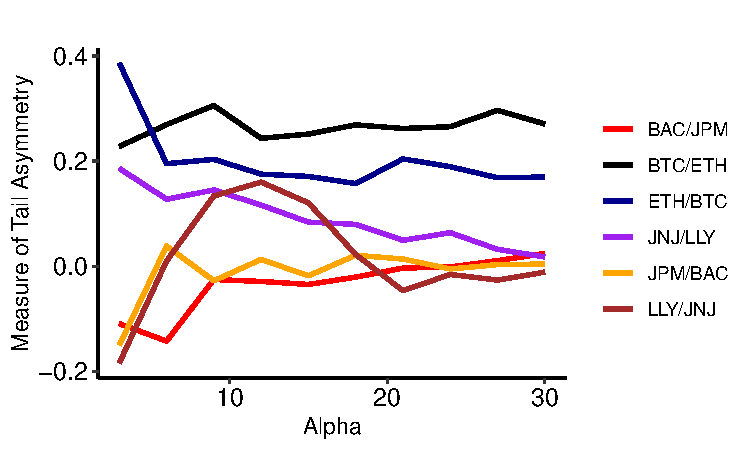
\includegraphics[width=0.55\linewidth]{Figures/6 pairs C-alpha.pdf}
\caption{Changes in the Asymmetry of Dependence Structures over the Tail Size}
\label{fig:fig1}
\end{figure}


Further examination also revealed that as the tail criterion, $\alpha$, rises the absolute value of $\mathbb{C}^i_{ij}$ in the equity market falls strongly while this is not the case in  cryptocurrencies. For instance, as table \ref{tab:illus} shows, when $\alpha$ rises from 3 to 10, the average of the absolute value of CQCD, $|\mathbb{C}^i_{ij}|$, in equity pairs falls from $0.15$ to $0.07$. This pattern continues as the value of $\alpha$ rises. This is more evident in figure \ref{fig:fig1}. With the rise in the threshold, $\alpha$, tail asymmetry among equity pairs converges to zero while in cryptocurrency pairs, this asymmetry persists even for much higher values of $\alpha$. In other words, in the equity market, the disparity between left-tail and right-tail correlations is mostly found when we only consider extreme events on each tail. The inclusion of less extreme events in the analysis, which happens by increasing the tail criterion, noticeably weakens this asymmetry. This is while tail asymmetry remains significant in both cryptocurrency pairs for larger values of $\alpha$. This is our second finding in this paper.

\subsection{Patterns of Asymmetry Across Markets}\label{sec:patt}
Building on the suggestive evidence in the previous section, this section establishes both patterns with the entire market data. Because our measures of tail dependence are not symmetric, we examine \(2 \times \binom{5}{2} = 20\) pairs in each equity sector -a total of $20 \times 11 = 220$ pairs- and \(2 \times \binom{10}{2} = 90\) pairs in the cryptocurrency market. Figure \ref{fig:hist} shows the distribution of conditional correlations on each tail as well as the difference between them, which is our measure of tail asymmetry (CQCD), for all pairs in both markets when the tail criterion is $\alpha = 5$. Figure \ref{fig:hist-sub3} confirms that the conditional tail asymmetry is stronger in cryptocurrencies. For instance, one can visually compare the mean of the distribution of CQCD in cryptocurrencies with its mean in the equity market. To further establish this pattern, table \ref{tab:pat-1} reports the industry-specific averages of measures of tail dependence for different values of $\alpha$. When $\alpha = 5$, the average CQCD between cryptocurrencies, $0.30$, is markedly greater than its average in the equity market, nearly $0.02$.

\begin{figure}[H]
\centering
\begin{subfigure}{.33\textwidth}
  \centering
  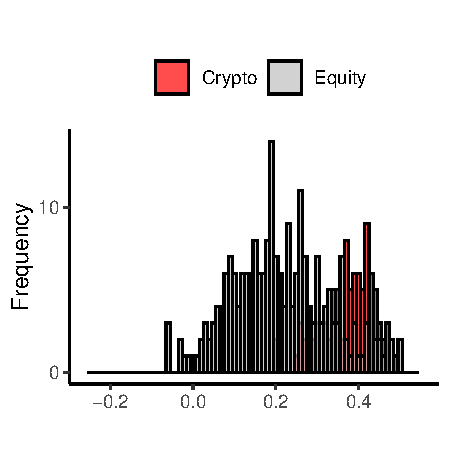
\includegraphics[width=\linewidth]{Figures/hist_lower.pdf}
  \caption{Left-tail}
  \label{fig:hist-sub1}
\end{subfigure}%
\begin{subfigure}{.33\textwidth}
  \centering
  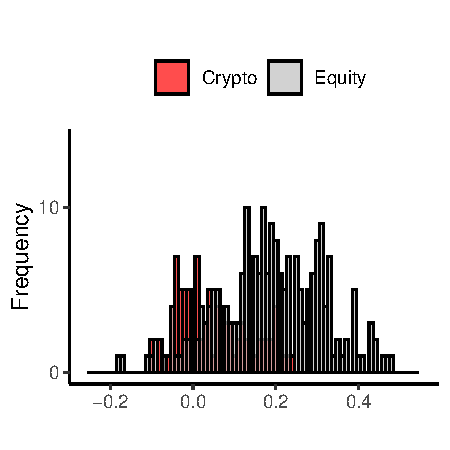
\includegraphics[width=\linewidth]{Figures/hist_upper.pdf}
  \caption{Right-tail}
  \label{fig:hist-sub2}
\end{subfigure}%
\begin{subfigure}{.33\textwidth}
  \centering
  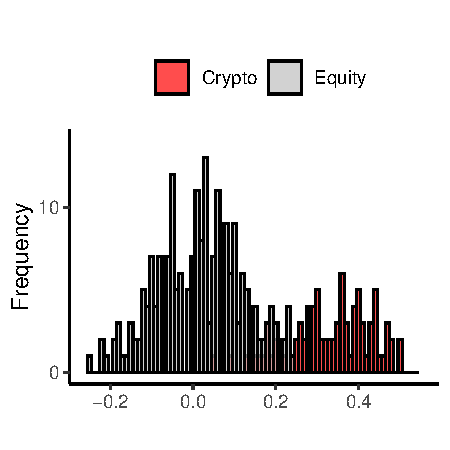
\includegraphics[width=\linewidth]{Figures/hist_d.pdf}
  \caption{CQCD}
  \label{fig:hist-sub3}
\end{subfigure}
\caption{Histograms of Conditional Tail Correlations in Equities vs. Cryptocurrencies ($\alpha = 5$)}
\label{fig:hist}
\end{figure}

 
The mechanism that generates this difference may be seen in histograms \ref{fig:hist-sub1} and \ref{fig:hist-sub2}, as well as in table \ref{tab:pat-1}. Overall, left-tail conditional correlations are stronger in the cryptocurrency market while right-tail correlations are stronger in the equity market. Thus, their difference, which is our measure of tail asymmetry, is significantly greater in the cryptocurrency market. Notably, in equity sectors where left-tail correlations are strong -\textit{e.g.,} energy- right-tail correlations are also equally strong. As a results their difference remains relatively small.
 
 

\begin{table}[H]\centering
\scriptsize
\caption{Asymmetry of Conditional Tail Dependence Structures Across Markets}\label{tab:pat-1}
\begin{threeparttable}
\begin{tabular}{lccccccccccccc}\toprule
 \multirow{3}{*}{Sector}  & &\multicolumn{3}{c}{$\alpha = 3$} & &\multicolumn{3}{c}{$\alpha = 5$} & &\multicolumn{3}{c}{$\alpha = 10$} \\\cmidrule{3-5}\cmidrule{7-9}\cmidrule{11-13}
 & & $\tilde{\tau}^{i,-}_{ij}(\alpha)$ & $\tilde{\tau}^{i,+}_{ij}(\alpha)$ & $\mathbb{C}^i_{ij}(\alpha)$ & & $\tilde{\tau}^{i,-}_{ij}(\alpha)$ & $\tilde{\tau}^{i,+}_{ij}(\alpha)$ & $\mathbb{C}^i_{ij}(\alpha)$ & & $\tilde{\tau}^{i,-}_{ij}(\alpha)$ & $\tilde{\tau}^{i,+}_{ij}(\alpha)$ & $\mathbb{C}^i_{ij}(\alpha)$   \\\midrule
& & & & & & \\[-2mm]
\multicolumn{1}{l}{Cryptocurrency}     &  & 0.3470 & 0.0421 & 0.3050 & & 0.3610 & 0.0617 & 0.3000 & & 0.3780 & 0.1170 & 0.2610  \\[1.25mm]
\multicolumn{1}{l}{Communications}     &  & 0.1220 & -0.0058 & 0.1280 & & 0.1030 & 0.0579 & 0.0454 & & 0.1310 & 0.1150 & 0.0156 \\
\multicolumn{1}{l}{Consumer Discretionary}     &  & 0.1390 & 0.0631 & 0.0762 & & 0.1550 & 0.0538 & 0.1010 & & 0.1600 & 0.0709 & 0.0888 \\
\multicolumn{1}{l}{Consumer Staples}     &  & 0.2040 & 0.2140 & -0.0091 & & 0.2410 & 0.1670 & 0.0742 & & 0.2050 & 0.1530 & 0.0523 \\
\multicolumn{1}{l}{Energy}     &  & 0.3210 & 0.3570 & -0.0361 & & 0.3450 & 0.3140 & 0.0308 & & 0.3160 & 0.2880 & 0.0281 \\
\multicolumn{1}{l}{Financials}   &  & 0.2670 & 0.3130 & -0.0461 & & 0.3210 & 0.3300 & -0.0093 & & 0.3290 & 0.2940 & 0.0356 \\
\multicolumn{1}{l}{Health Care}   &  & 0.1450 & 0.1560 & -0.0105 & & 0.1140 & 0.1630 & -0.0494 & & 0.1570 & 0.1570 & -0.0009 \\
\multicolumn{1}{l}{Industrials}     &  & 0.0659 & 0.1330 & -0.0670 & & 0.1220 & 0.1380 & -0.0163 & & 0.1600 & 0.1880 & -0.0287 \\
\multicolumn{1}{l}{Materials}     &  & 0.1240 & 0.1040 & 0.0198 & & 0.1620 & 0.1350 & 0.0272 & & 0.2010 & 0.1820 & 0.0192 \\
\multicolumn{1}{l}{Real Estate}     &  & 0.1960 & 0.2420 & -0.0464 & & 0.2050 & 0.2230 & -0.0178 & & 0.2000 & 0.2240 & -0.0231 \\
\multicolumn{1}{l}{Technology}     &  & 0.1560 & 0.1690 & -0.0128 & & 0.2250 & 0.2030 & 0.0222 & & 0.2660 & 0.2000 & 0.0656 \\
\multicolumn{1}{l}{Utilities}     &  & 0.3220 & 0.3450 & -0.0233 & & 0.3130 & 0.3030 & 0.0099 & & 0.2880 & 0.2850 & 0.0024 \\
\bottomrule
\end{tabular}
%\begin{tablenotes}      
%\item Note: This table presents a summary of our tail analysis in each sector with an emphasis on the asymmetry as measured by the CQCD ($\mathbb{C}^i_{ij}(\alpha)$) statistic over different values of $\alpha$. 
%\end{tablenotes}
\end{threeparttable}
\end{table}

To illustrate the second pattern, table \ref{tab:asym} shows how the share of pairs with a 'small' tail asymmetry changes with the tail criterion. More precisely, in each sector, we report the proportion of pairs where the absolute value of CQCD is less than $0.05$ or $0.10$. Consistent with our previous finding, the share of such pairs is significantly larger in the equity market. For instance, when $\alpha = 5$ the fraction of cryptocurrencies whose CQCD is less than $0.10$ is nearly half of one percent while the average across the equities is more than $58$\%. More importantly, as $\alpha$ rises, this proportion among the equities noticeably increases so much so that when $\alpha = 30$, the value of CQCD in more than $85$\% of equity pairs is less than $0.10$. On the contrary, the tail asymmetry in almost all of cryptocurrency pairs remains greater than $0.10$ at $\alpha = 30$, or even beyond that at $\alpha = 50$. Thus, we conclude that conditional tail asymmetry in the equity market is mostly limited to the tails with extreme returns while in cryptocurrencies, it is found throughout the joint distribution of returns. 


\begin{table}[H]\centering
\scriptsize
\caption{Proportion of Small Tail Asymmetries in Equities vs. Cryptocurrencies (\%)}\label{tab:asym}
\begin{threeparttable}
\begin{tabular}{lcccccccccc}\toprule
 \multirow{3}{*}{Sector}  & &\multicolumn{2}{c}{$\alpha = 5$}  & &\multicolumn{2}{c}{$\alpha = 15$} & &\multicolumn{2}{c}{$\alpha = 30$} \\\cmidrule{3-4}\cmidrule{6-7}\cmidrule{9-10}
 & & $  \big\lvert \mathbb{C} \big\rvert  < 0.05 $   & $\big\lvert \mathbb{C} \big\rvert  < 0.10 $ & &  $  \big\lvert \mathbb{C} \big\rvert  < 0.05 $   & $\big\lvert \mathbb{C} \big\rvert  < 0.10 $ & &  $  \big\lvert \mathbb{C} \big\rvert  < 0.05 $   & $\big\lvert \mathbb{C} \big\rvert  < 0.10 $   \\\midrule
& & & & & & \\[-2mm]
\multicolumn{1}{l}{Cryptocurrency}   & & 0.47 & 0.95 & & 0 & 0.47 & & 0 & 0 \\[1.25mm]
\multicolumn{1}{l}{Communications}    & & 25 & 60 & & 45 & 60 & & 80 & 95 \\
\multicolumn{1}{l}{Consumer Discretionary}    & & 10 & 35 & & 40 & 60 & & 50 & 75 \\
\multicolumn{1}{l}{Consumer Staples}  & & 25 & 55 & & 70 & 85 & & 65 & 80 \\
\multicolumn{1}{l}{Energy}           & & 45 & 75 & & 60 & 85 & & 80 & 100 \\
\multicolumn{1}{l}{Financials}       & & 40 & 55 & & 55 & 95 & & 40 & 80 \\
\multicolumn{1}{l}{Health Care}      & & 25 & 55 & & 50 & 85 & & 60 & 95 \\
\multicolumn{1}{l}{Industrials }    & & 30 & 70 & & 70 & 85 & & 85 & 95 \\
\multicolumn{1}{l}{Materials}        & & 25 & 45 & & 65 & 90 & & 55 & 95 \\
\multicolumn{1}{l}{Real Estate}      & & 15 & 40 & & 90 & 90 & & 65 & 90 \\
\multicolumn{1}{l}{Technology}       & & 40 & 75 & & 30 & 50 & & 5 & 20 \\
\multicolumn{1}{l}{Utilities}       & & 45 & 70 & & 35 & 80 & & 85 & 100 \\
\bottomrule
\end{tabular}
\begin{tablenotes}      
\item Note: For each of $\alpha$, the value of our measure of tail asymmetry is computed for all distinct pairs in each sector. This table reports the percentage of the pairs whose CQCD ($\mathbb{C}$) statistic is close to zero. It is evident that this share is rising with $\alpha$ in the equity market while it's negligible in the cryptocurrency market. 
\end{tablenotes}
\end{threeparttable}
\end{table}


\subsection{Parametric Bootstraps}
Our parametric bootstraps follow the algorithm in section \ref{sec:boot}. We, first, fit a bivariate copula to capture the joint distribution of returns.\footnote{We run this step for all 310 pairs individually. In the interest of brevity, we do not report the results in the paper but they are available upon request.} Then we construct random samples form the fitted copulas. For each pair, these simulated samples have the same size of the associated observed sample in the data. We compute measures of tail asymmetry in each simulated sample and repeat this process $5000$ times. This results in bootstrap-generated distributions of CQCD in each pair. As an example, figure \ref{fig:cqds:boot} shows this distribution at $\alpha = 5$ for three pairs. As evident, the mean of this distribution in the cryptocurrency pair (\ref{fig:boot-sub1}) is considerably greater than the mean of equity pairs (figures \ref{fig:boot-sub2} and \ref{fig:boot-sub3}). 


\begin{figure}[H]
    \centering
    \begin{subfigure}[b]{0.3\textwidth}  % Adjust the width to fit your document layout
        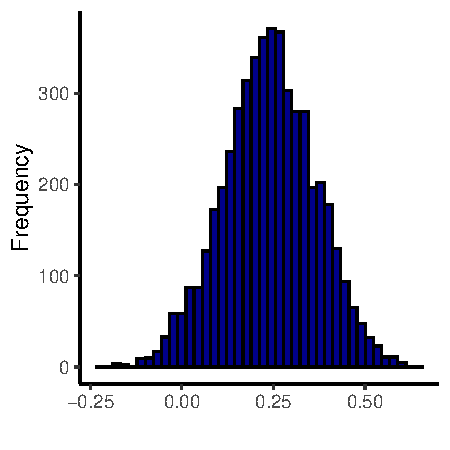
\includegraphics[width=\textwidth]{Figures/hist_BTC_ETH.pdf}
        \caption{(BTC, ETH)}
        \label{fig:boot-sub1}
    \end{subfigure}
    % Remove line breaks to place figures in a row
    \begin{subfigure}[b]{0.3\textwidth}
        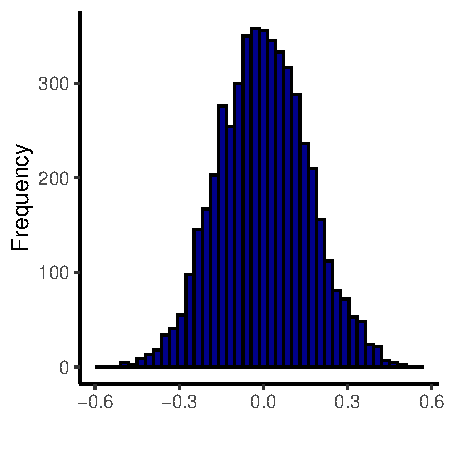
\includegraphics[width=\textwidth]{Figures/hist_LLY_JNJ.pdf}
        \caption{(LLY, JNJ)}
        \label{fig:boot-sub2}
    \end{subfigure}
    \begin{subfigure}[b]{0.3\textwidth}
        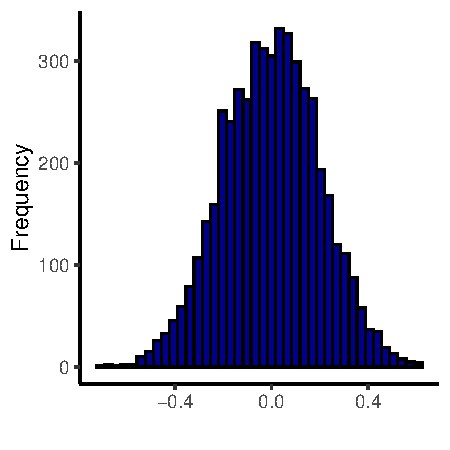
\includegraphics[width=\textwidth]{Figures/hist_JPM_BAC.pdf}
        \caption{(JPM, BAC)}
        \label{fig:boot-sub3}
    \end{subfigure}
    \caption{Distributions of CQCD  for Sample Pairs ($\alpha =5$)}
    \label{fig:cqds:boot}
\end{figure}



 Table \ref{tab:boots} compares the average of mean and standard deviations of bootstrapped CQCDs across all sectors, which confirm that tail asymmetry is consistently larger in cryptocurrencies. For each pair, we also compute the quantile of this distribution for which tail asymmetry fades away -\textit{i.e.,} $\mathbb{C} = 0$. Table \ref{tab:boots} reports industry averages of this quantile at $\alpha = 5$ and $\alpha = 10$. The distribution of CQCD in equities is almost perfectly centered at zero as this quantile is almost exactly in the middle of the distribution. On the contrary, in cryptocurrencies, the average quantile where tail asymmetry is negligible is noticeably smaller, which confirms our first finding. 
 

\begin{table}[H]\centering
\scriptsize
\caption{Bootstraps of Conditional Tail Asymmetries}\label{tab:boots}
\begin{threeparttable}
\begin{tabular}{lcccccccccccc}\toprule
\multirow{3}{*}{Sector}  & & \multicolumn{5}{c}{$\alpha = 5$} & & \multicolumn{5}{c}{$\alpha = 10$}
\\\cmidrule{3-7}\cmidrule{9-13}
 & & $\mathbb{E}\big[\mathbb{C}\big]$ & & Sd\big($\mathbb{C}$\big) &  & $\mathbb{E}\Big[q\big(\mathbb{C} = 0\big)\Big]$ & & $\mathbb{E}\big[\mathbb{C}\big]$ & & Sd\big($\mathbb{C}$\big) &  & $\mathbb{E}\Big[q\big(\mathbb{C} = 0\big)\Big]$
 \\\midrule
& & & & & & \\[-2mm]
\multicolumn{1}{l}{Cryptocurrency}            &  & 0.156 & & 0.123  & & 0.139 & & 0.178 & & 0.084 & & 0.103  \\[1.5mm]
\multicolumn{1}{l}{Communications}            &  & 0.027 & & 0.156  & & 0.426 & & 0.031 & & 0.110 & & 0.393  \\
\multicolumn{1}{l}{Consumer Discretionary}    &  & 0.043 & & 0.153  & & 0.389 & & 0.049 & & 0.109 & & 0.331  \\
\multicolumn{1}{l}{Consumer Staples}          &  & 0.003 & & 0.157  & & 0.491 & & 0.006 & & 0.110 & & 0.478  \\
\multicolumn{1}{l}{Energy}                    &  & 0.000 & & 0.165  & & 0.500 & & 0.000 & & 0.112 & & 0.501  \\
\multicolumn{1}{l}{Financials}                &  & 0.009 & & 0.167  & & 0.472 & & 0.012 & & 0.115 & & 0.452  \\
\multicolumn{1}{l}{Health Care}               &  & 0.003 & & 0.158  & & 0.496 & & 0.001 & & 0.111 & & 0.495  \\
\multicolumn{1}{l}{Industrials }              &  & 0.000 & & 0.159  & & 0.501 & & 0.000 & & 0.111 & & 0.499  \\
\multicolumn{1}{l}{Materials}                 &  & 0.011 & & 0.157  & & 0.471 & & 0.014 & & 0.110 & & 0.452  \\
\multicolumn{1}{l}{Real Estate}               &  & 0.002 & & 0.159  & & 0.500 & & 0.000 & & 0.111 & & 0.500  \\
\multicolumn{1}{l}{Technology}                &  & 0.036 & & 0.152  & & 0.402 & & 0.044 & & 0.107 & & 0.342  \\
\multicolumn{1}{l}{Utilities}                 &  & 0.010 & & 0.154  & & 0.469 & & 0.009 & & 0.107 & & 0.460  \\
\bottomrule
\end{tabular}
\begin{tablenotes}      
\item Note: This table presents a summary of our bootstrap simulations in each sector. After fitting bivariate copulas to each pair of assets, random sample was constructed and measures of tail asymmetry were computed. This process was repeated for $n=5000$ time, which resulted in a distribution of CQCD's in each sector. This table reports some moments of this distribution in each sector for $\alpha = 5$ and $\alpha = 10$.    
\end{tablenotes}
\end{threeparttable}
\end{table}

As for the second pattern, figure \ref{fig:boot2} shows the proportion of pairs with small ($<0.05$) or large ($>0.10$) tail asymmetries in each sector in our bootstraps. Figure \ref{fig:boot2-sub1} shows that as the tail criterion rises, the proportion of pairs with a small tail asymmetry ($<0.05$) in the equity market steadily rises while in cryptocurrencies it all but falls. At the same time, the share of pairs with large CQCDs ($>0.10$) unambiguously falls in all equity sectors while the rise of $\alpha$ has almost no impact on the portion of cryptocurrency pairs with large tail asymmetries (fig. \ref{fig:boot2-sub2}). In other words, including less extreme returns significantly weakens tail asymmetry in the equities while it doesn't affect the cryptocurrencies, which confirms our second finding. 


\begin{figure}[H]
    \centering
    \begin{subfigure}[b]{0.45\textwidth}  % Adjust the width to fit your document layout
        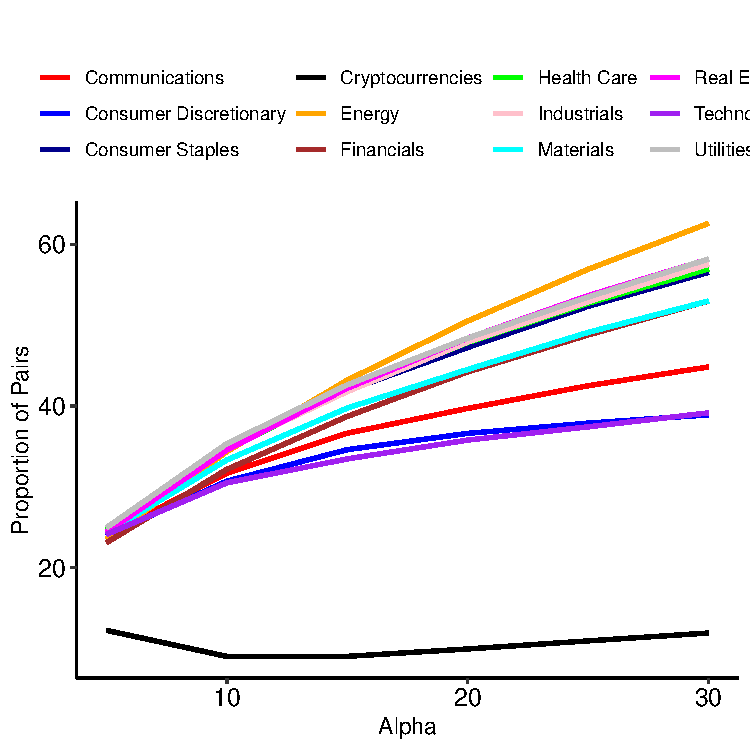
\includegraphics[width=\textwidth]{Figures/CQCD_5.pdf}
        \caption{$\big\lvert\mathbb{C}\big\rvert < 0.05$}
        \label{fig:boot2-sub1}
    \end{subfigure}
    % Remove line breaks to place figures in a row
    \begin{subfigure}[b]{0.45\textwidth}
        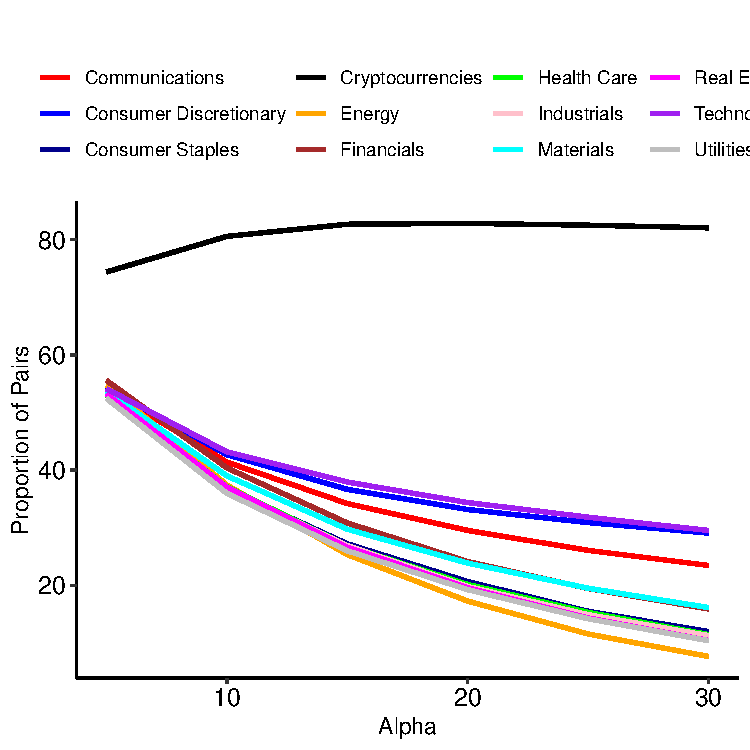
\includegraphics[width=\textwidth]{Figures/CQCD_10.pdf}
       \caption{$\big\lvert\mathbb{C}\big\rvert > 0.10$}
        \label{fig:boot2-sub2}
    \end{subfigure}
    \caption{Proportion of Pairs (\%) with Small and Large Tail Asymmetries in Bootstraps}
    \label{fig:boot2}
\end{figure}




\section{Conclusion}\label{con}
We study the asymmetry of tail dependence structures in both the equity and cryptocurrency market. While it is known that financial assets are more strongly correlated during the downfalls, our results uncover two differences in the nature of tail dependence structures in these two markets. We find that (1) the asymmetry of tail correlations is significantly stronger between cryptocurrencies. We show this pattern by introducing a measure of asymmetry, which we call Conditional Quantile Correlation Difference (CQCD). What causes this disparity in the markets is that, overall, left-tail correlations tend to be stronger in cryptocurrencies while right-tail correlations are stronger in the equity market. We also show that (2) this asymmetry in the equity market is mostly limited to the tails that only include extreme events. We find that increasing the tail criterion leads to a noticeable fall in the value of CQCD in the equities. In cryptocurrencies, however, the asymmetry is observed throughout the entire joint distribution of returns. \par

\vspace{2mm}
\noindent\textbf{Acknowledgments} \par
We would like to thank Arash A. Amini for his insightful suggestions. 

%segmented correlation matrix

%\begin{itemize}
%\item F ENG , W., WANG , Y. and Z HANG , Z. (2018). Can cryptocurrencies be a safe haven: A tail risk perspective
%analysis. Appl. Econ. 50 4745–4762
%\item The Annals of Applied Statistics, 2022, Vol. 16, No. 3, 1822–1847
%https://doi.org/10.1214/21-AOAS1568, Institute of Mathematical Statistics, 2022,
%ASYMMETRIC TAIL DEPENDENCE MODELING, WITH APPLICATION TO CRYPTOCURRENCY MARKET DATA
%B Y YAN G ONG a AND R APHAeL H USER
%\item 
%\item Han, H., Linton, O., Oka, T., \& Whang, Y. J. (2016). The cross-quantilogram: measuring quantile dependence and testing directional predictability between time series. Journal of Econometrics, 193(1), 251–270.
%\item \cite{Georgoula2015, corbet2018}
%\end{itemize}

\bibliographystyle{plainnat}
\bibliography{refs_1}

\section*{Appendix}\label{app}
\vspace{-8mm}
\begin{table}[H]\centering
\scriptsize
\caption{Descriptive Statistics of Return Series}\label{tab:sum}
\begin{threeparttable}
\begin{tabular}{p{1.75cm}p{3.5cm}lcccccccc}
\toprule
Sector & Name & Ticker & N & Mean & std. & Min & Max & Skewness & Kurtosis \\
\midrule 
\multicolumn{2}{l}{Cryptocurrency}\\[1mm]
& Bitcoin            & BTC & 2379 & 0.001 & 0.038 & -0.465 & 0.225 & -0.793 & 15.800 \\
& Ethereum           & ETH & 2379 & 0.001 & 0.047 & -0.551 & 0.235 & -0.926 & 14.000 \\
& Binance Coin       & BNB & 2379 & 0.002 & 0.054 & -0.543 & 0.529 & 0.407  & 20.400 \\
& Ripple             & XRP & 2379 & 0.000 & 0.059 & -0.551 & 0.607 & 1.140  & 23.400 \\
& Cardano            & ADA & 2379 & 0.001 & 0.062 & -0.504 & 0.862 & 1.970  & 30.000 \\
& Chainlink          & LINK& 2379 & 0.002 & 0.065 & -0.615 & 0.481 & -0.066 & 11.000 \\
& Bitcoin Cash       & BCH & 2379 & 0.000 & 0.061 & -0.561 & 0.460 & 0.292  & 15.500 \\
& EOS                & EOS & 2379 & 0.000 & 0.061 & -0.504 & 0.440 & -0.083 & 12.300 \\
& Stellar            & XLM & 2379 & 0.000 & 0.057 & -0.410 & 0.559 & 1.030  & 16.600 \\
& Neo                & NEO & 2379 & 0.000 & 0.059 & -0.466 & 0.346 & -0.247 & 9.710  \\
\multicolumn{2}{l}{Communications}\\[1mm]
& Comcast Corp.           & CMCSA  & 1636 & 0.000 & 0.017 & -0.096 & 0.118 & -0.247 & 8.270 \\
& Verizon Communications  & VZ     & 1636 & 0.000 & 0.013 & -0.078 & 0.089 & 0.022 & 8.840 \\
& T-Mobile US Inc.        & TMUS   & 1636 & 0.001 & 0.017 & -0.119 & 0.111 & 0.130 & 11.300 \\
& The Walt Disney Company & DIS    & 1636 & 0.000 & 0.020 & -0.141 & 0.135 & 0.063 & 12.300 \\
& Netflix Inc.            & NFLX   & 1636 & 0.001 & 0.029 & -0.433 & 0.156 & -2.140 & 37.000 \\
\multicolumn{2}{l}{Consumer Discretionary }  \\[1mm]
& Tesla Inc.         & TSLA & 1636 & 0.001 & 0.040 & -0.237 & 0.181 & -0.120 & 6.720 \\
& Amazon.com Inc.    & AMZN & 1636 & 0.001 & 0.022 & -0.151 & 0.127 & -0.131 & 7.080 \\
& Home Depot         & HD   & 1636 & 0.001 & 0.017 & -0.221 & 0.129 & -1.490 & 25.500 \\
& Nike               & NKE  & 1636 & 0.000 & 0.020 & -0.137 & 0.144 & -0.024 & 12.100 \\
& McDonald's Corp    & MCD  & 1636 & 0.000 & 0.014 & -0.173 & 0.167 & -0.288 & 35.500 \\
\multicolumn{2}{l}{Consumer Staples}\\[1mm]
& Procter \& Gamble   & PG  & 1636 & 0.000 & 0.013 & -0.091 & 0.113 & 0.020  & 14.600 \\
& Coca-Cola Co.       & KO  & 1636 & 0.000 & 0.013 & -0.102 & 0.063 & -0.939 & 13.200 \\
& PepsiCo             & PEP & 1636 & 0.000 & 0.013 & -0.121 & 0.122 & -0.603 & 23.900 \\
& Costco Wholesale    & COST& 1636 & 0.001 & 0.015 & -0.133 & 0.095 & -0.485 & 12.400 \\
& Walmart Inc.        & WMT & 1636 & 0.000 & 0.014 & -0.121 & 0.111 & -0.197 & 19.200 \\
\multicolumn{2}{l}{Energy}\\[1mm]
& Exxon Mobil Corp.  & XOM & 1636 & 0.000 & 0.020 & -0.130 & 0.119 & -0.179 & 8.450 \\
& Chevron Corp.      & CVX & 1636 & 0.000 & 0.021 & -0.250 & 0.205 & -1.070 & 29.000 \\
& ConocoPhillips     & COP & 1636 & 0.001 & 0.026 & -0.286 & 0.225 & -0.641 & 19.300 \\
& EOG Resources      & EOG & 1636 & 0.000 & 0.028 & -0.386 & 0.153 & -1.450 & 26.500 \\
& Occidental Petroleum & OXY & 1636 & 0.000 & 0.037 & -0.734 & 0.290 & -4.130 & 97.800 \\
\multicolumn{2}{l}{ Financials}   \\[1mm]
& Visa Inc.          & V    & 1636 & 0.001 & 0.017 & -0.146 & 0.130 & -0.071 & 12.500 \\
& JPMorgan Chase     & JPM  & 1636 & 0.001 & 0.019 & -0.162 & 0.166 & -0.100 & 16.600 \\
& Mastercard         & MA   & 1636 & 0.001 & 0.019 & -0.136 & 0.154 & 0.012  & 11.100 \\
& Bank of America    & BAC  & 1636 & 0.000 & 0.021 & -0.167 & 0.164 & -0.004 & 13.500 \\
& Wells Fargo        & WFC  & 1636 & 0.000 & 0.022 & -0.173 & 0.136 & -0.343 & 11.000 \\
\multicolumn{2}{l}{Healthcare}   \\[1mm]         
& Eli Lilly and Co   & LLY  & 1636 & 0.001 & 0.018 & -0.105 & 0.146 & 1.010 & 13.300 \\
& Johnson \& Johnson & JNJ  & 1636 & 0.000 & 0.013 & -0.106 & 0.077 & -0.441 & 12.800 \\
& UnitedHealth Group & UNH  & 1636 & 0.001 & 0.018 & -0.190 & 0.120 & -0.482 & 17.400 \\
& Merck \& Co.       & MRK  & 1636 & 0.001 & 0.014 & -0.104 & 0.080 & -0.209 & 9.640 \\
& AbbVie             & ABBV & 1636 & 0.000 & 0.017 & -0.177 & 0.129 & -1.280 & 19.500 \\
\multicolumn{2}{l}{Industrials}   \\[1mm]
& UPS                 & UPS  & 1636 & 0.000 & 0.018 & -0.105 & 0.134 & 0.276  & 11.300 \\
& Union Pacific Corp. & UNP  & 1636 & 0.001 & 0.017 & -0.140 & 0.122 & -0.295 & 13.400 \\
& Caterpillar Inc.    & CAT  & 1636 & 0.001 & 0.020 & -0.154 & 0.098 & -0.465 & 7.470  \\
& Boeing              & BA   & 1636 & 0.000 & 0.030 & -0.272 & 0.218 & -0.440 & 17.200 \\
& Honeywell International & HON & 1636 & 0.000 & 0.016 & -0.129 & 0.140 & -0.215 & 14.100 \\
\multicolumn{2}{l}{Materials}\\[1mm]
& Linde              & LIN & 1636 & 0.001 & 0.016 & -0.109 & 0.111 & -0.091 & 8.830 \\
& Sherwin-Williams   & SHW & 1636 & 0.001 & 0.018 & -0.207 & 0.135 & -0.757 & 18.700 \\
& Freeport-McMoRan   & FCX & 1636 & 0.001 & 0.031 & -0.199 & 0.260 & -0.153 & 8.890 \\
& Ecolab             & ECL & 1636 & 0.000 & 0.018 & -0.125 & 0.200 & 0.122  & 20.600 \\
& Air Products and Chemicals & APD & 1636 & 0.000 & 0.018 & -0.169 & 0.129 & -1.190 & 18.200 \\[1mm]
\multicolumn{2}{l}{ Real Estate} \\[1mm]
& Prologis           & PLD  & 1636 & 0.000 & 0.018 & -0.190 & 0.112 & -0.727 & 14.300 \\
& American Tower     & AMT  & 1636 & 0.000 & 0.018 & -0.164 & 0.115 & -0.087 & 12.000 \\
& Crown Castle       & CCI  & 1636 & 0.000 & 0.017 & -0.133 & 0.107 & -0.185 & 9.200 \\
& Simon Property Group & SPG & 1636 & 0.000 & 0.027 & -0.311 & 0.246 & -1.010 & 30.900 \\
& Equinix            & EQIX & 1636 & 0.000 & 0.018 & -0.135 & 0.110 & 0.040  & 8.390 \\
\multicolumn{2}{l}{Technology}  \\[1mm]
& Microsoft Corp.    & MSFT & 1636 & 0.001 & 0.019 & -0.159 & 0.133 & -0.242 & 10.000 \\      
& Apple Inc.         & AAPL & 1636 & 0.001 & 0.020 & -0.138 & 0.113 & -0.217 & 8.190 \\
& Alphabet Inc.      & GOOG & 1636 & 0.001 & 0.020 & -0.118 & 0.099 & -0.220 & 7.170 \\
& NVIDIA Corporation & NVDA & 1636 & 0.002 & 0.032 & -0.208 & 0.218 & -0.164 & 7.720 \\
& Meta Platforms     & META & 1636 & 0.001 & 0.027 & -0.306 & 0.209 & -1.360 & 27.000 \\
\multicolumn{2}{l}{Utilities}\\[1mm]
& NextEra Energy     & NEE & 1636 & 0.001 & 0.017 & -0.144 & 0.128 & -0.453 & 13.300 \\
& Duke Energy        & DUK & 1636 & 0.000 & 0.014 & -0.122 & 0.116 & -0.195 & 17.000 \\
& Southern Co.       & SO  & 1636 & 0.000 & 0.015 & -0.125 & 0.172 & 0.263  & 23.600 \\
& Dominion Energy    & D   & 1636 & 0.000& 0.016 & -0.131 & 0.159 & -0.419 & 19.400 \\
& Exelon Corp.       & EXC & 1636 & 0.000 & 0.017 & -0.175 & 0.165 & -0.285 & 24.000 \\
\bottomrule
\end{tabular}
\begin{tablenotes}      
\item Note: This table reports the descriptive statistics of log daily returns of assets in our sample from 9 Nov. 2017 to 15 May 2024.
\end{tablenotes}
\end{threeparttable}
\end{table}






\end{document}
